\documentclass{article} % A4 paper and 11pt font size
\setcounter{secnumdepth}{0}

\usepackage{amssymb, amsmath, amsfonts}
\usepackage{moreverb}
\usepackage{graphicx}
\usepackage{enumerate}
\usepackage{graphics}
\usepackage[margin=1in]{geometry}
\usepackage{color}
\usepackage{tocloft}
\renewcommand{\cftsecleader}{\cftdotfill{\cftdotsep}}
\usepackage{array}
\usepackage{float}
\usepackage{csquotes}
\usepackage{verbatim}
\usepackage{hyperref}
\usepackage{textcomp}
\usepackage[makeroom]{cancel}
\usepackage{bbold}
\usepackage{scrextend}
\usepackage{alltt}
\usepackage{listings}
\usepackage{physics}
\usepackage{mathtools}
\usepackage[normalem]{ulem}
\usepackage{amsthm}
\usepackage{tikz}
\usetikzlibrary{positioning}
\usetikzlibrary{arrows}
\usepackage{pgfplots}
\usepackage{bigints}
\allowdisplaybreaks
\pgfplotsset{compat=1.12}

\theoremstyle{plain}
\newtheorem*{theorem*}{Theorem}
\newtheorem{theorem}{Theorem}
\newtheorem*{lemma*}{Lemma}
\newtheorem{lemma}{Lemma}

\definecolor{verbgray}{gray}{0.9}
% \definecolor{dkgreen}{green}{0.9}

\lstnewenvironment{code}{%
  \lstset{
  language=Python,
  backgroundcolor=\color{verbgray},
  keywordstyle=\color{blue},      % keyword style
  keywordstyle=[2]\color{blue},   % keyword style
  commentstyle=\color{magenta},   % comment style
  stringstyle=\color{olive},      % string literal styleframe=single,
  numberstyle=\color{black},      % string literal styleframe=single,
  framerule=0pt,
  numbers=left,
  stepnumber=1,
  firstnumber=1,
  showspaces=false,
  basicstyle=\ttfamily}}{}

\lstnewenvironment{console_output}{%
  \lstset{
  framerule=0pt,
  numbers=left,
  stepnumber=1,
  showspaces=false,
  firstnumber=1,
  basicstyle=\ttfamily}}{}


\makeatletter
\newcommand{\BIGG}{\bBigg@{3}}
\newcommand{\vast}{\bBigg@{4}}
\newcommand{\Vast}{\bBigg@{5}}
\makeatother

\newenvironment{definition}[1][Definition]{\begin{trivlist}
\item[\hskip \labelsep {\bfseries #1}]}{\end{trivlist}}

\newcommand{\dy}{\partial_y}
\newcommand{\dyy}{\partial_{yy}}
\newcommand{\dxx}{\partial_{xx}}
\newcommand{\dxy}{\partial_{xy}}
\newcommand{\dyyy}{\partial_{yyy}}
\newcommand{\dxxx}{\partial_{xxx}}
\newcommand{\dx}{\partial_x}
\newcommand{\E}{\varepsilon}
\def\Rl{\mathbb{R}}
\def\Cx{\mathbb{C}}

\newcommand{\Ei}{\text{Ei}}

\usepackage[T1]{fontenc} % Use 8-bit encoding that has 256 glyphs
\usepackage{fourier} % Use the Adobe Utopia font for the document - comment this line to return to the LaTeX default
\usepackage[english]{babel} % English language/hyphenation

\usepackage{sectsty} % Allows customizing section commands
\allsectionsfont{\centering \normalfont\scshape} % Make all sections centered, the default font and small caps

\usepackage{fancyhdr} % Custom headers and footers
\pagestyle{fancy} % Makes all pages in the document conform to the custom headers and footers
\fancyhead[L]{\bf Sam Fleischer}
\fancyhead[C]{\bf UC Davis \\ Numerical Solutions of Differential Equations (MAT228A)} % No page header - if you want one, create it in the same way as the footers below
\fancyhead[R]{\bf Fall 2016}

\fancyfoot[L]{\bf } % Empty left footer
\fancyfoot[C]{\bf \thepage} % Empty center footer
\fancyfoot[R]{\bf } % Page numbering for right footer
\renewcommand{\headrulewidth}{0pt} % Remove header underlines
\renewcommand{\footrulewidth}{0pt} % Remove footer underlines
\setlength{\headheight}{25pt} % Customize the height of the header

\newcommand{\VEC}[2]{\left\langle #1, #2 \right\rangle}
\newcommand{\ran}{\text{\rm ran }}
\newcommand{\Hilb}{\mathcal{H}}
\newcommand{\lap}{\Delta}

\newcommand{\littleo}[1]{\text{\scriptsize$\mathcal{O}$}\qty(#1)}

\DeclareMathOperator*{\esssup}{\text{ess~sup}}

\newcommand{\problem}[2]{
\vspace{.375cm}
\boxed{\begin{minipage}{\textwidth}
    \section{\bf #1}
    #2
\end{minipage}}
}

\numberwithin{equation}{section} % Number equations within sections (i.e. 1.1, 1.2, 2.1, 2.2 instead of 1, 2, 3, 4)
\numberwithin{figure}{section} % Number figures within sections (i.e. 1.1, 1.2, 2.1, 2.2 instead of 1, 2, 3, 4)
\numberwithin{table}{section} % Number tables within sections (i.e. 1.1, 1.2, 2.1, 2.2 instead of 1, 2, 3, 4)

\setlength\parindent{0pt} % Removes all indentation from paragraphs - comment this line for an assignment with lots of text

\newcommand{\horrule}[1]{\rule{\linewidth}{#1}} % Create horizontal rule command with 1 argument of height

\title{ 
\normalfont \normalsize 
\textsc{UC Davis, Numerical Solutions of Differential Equations (MAT 228A), Fall 2016} \\ [25pt] % Your university, school and/or department name(s)
\horrule{2pt} \\[0.4cm] % Thin top horizontal rule
\Huge Homework \#1 \\ % The assignment title
\horrule{2pt} \\[0.5cm] % Thick bottom horizontal rule
}

\author{\huge Sam Fleischer} % Your name

\date{October 14, 2016} % Today's date or a custom date

\begin{document}\thispagestyle{empty}

\maketitle % Print the title

\makeatletter
\@starttoc{toc}
\makeatother

\pagebreak

%%%%%%%%%%%%%%%%%%%%%%%%%%%%%%%%%%%%%%
\problem{Problem 1}{Let $L$ be the linear operator $Lu = u_{xx}$, $u_x(0) = u_x(1) = 0$.
\begin{enumerate}[\ \ (a)]
    \item Find the eigenfunctions and corresponding eigenvalues of $L$.
    \item Show that the eigenfunctions are orthogonal in the $L^2[0,1]$ inner product $$\langle u, v \rangle = \int_0^1 u(x) v(x) \dd x.$$
    \item It can be shown that the eigenfunctions $\phi_j(x)$, form a complete set in $L^2[0,1]$. This means that for any $f \in L^2[0,1]$, $f(x) = \sum_{j} \alpha_j\phi_j(x)$.  Express the solution to $$u_{xx} = f, u_x(0)=u_x(1) = 0,$$ as a series solution of the eigenfunctions.
    \item Note that this BVP does not have a solution for all $f$.  Express the condition for existence of a solution in terms of the eigenfunctions of $L$.
\end{enumerate}}

\begin{enumerate}[\ \ (a)]
    \item
        Let $Lu = \lambda u$.  Then
        \begin{align*}
            u_{xx} - \lambda u = 0 \\
            \implies u(x) = A\exp[\sqrt{\lambda}x] + B\exp[-\sqrt{\lambda}x]
        \end{align*}
        If $\lambda > 0$ then $u_x(x) = \sqrt{\lambda}\qty[A\exp[\sqrt{\lambda}x] - B\exp[\sqrt{-\lambda}x]]$ and the boundary condition $u_x(0) = 0$ implies $A = B$ and so $u_x(x) = A\sqrt{\lambda}\qty[\exp[\sqrt{\lambda}x] - \exp[-\sqrt{\lambda}x]]$.  Then the boundary condition $u_x(1) = 0$ implies $A = 0$, thus there are no solutions.

        If $\lambda = 0$ then $u(x) = A + Bx$ and the boundary conditions implies $B = 0$.  Thus $u(x) = A$ where $A$ is a constant is an eigenfunction.

        If $\lambda < 0$ then $u(x) = A\sin(\sqrt{-\lambda}x) + B\cos(\sqrt{-\lambda}x)$ and thus $u_x(x) = \sqrt{-\lambda}\qty[A\cos(\sqrt{-\lambda}x) - B\sin(\sqrt{-\lambda}x)]$.  Then the boundary conditions imply $A = 0$ and $\sqrt{-\lambda} = k\pi$ for $k \in \mathbb{N}$.  Thus the eigenfunctions are
        \begin{align*}
            u_k(x) = \cos(k\pi x) \qquad \text{for $k = 0, 1, 2, \dots$ with corresponding eigenvalues } \lambda_k = -k^2\pi^2
        \end{align*}
    \item
        Assume $k \neq j$.  Then
        \begin{align*}
            \left\langle \cos(k \pi x), \cos(j \pi x) \right\rangle &= \int_0^1\cos(k\pi x)\cos(j\pi x)\dd x \\
            &= \frac{1}{2}\int_0^1\cos((k+j)\pi x) + \cos((k-j)\pi x)\dd x \\
            &= \frac{1}{2}\qty[\left.\frac{\sin(k+j)\pi x}{(k+j)\pi}\right|_0^1 + \left.\frac{\sin(k-j)\pi x}{(k-j)\pi}\right|_0^1] \\
            &= \frac{1}{2(k+j)\pi}\qty[\sin(k+j)\pi] + \frac{1}{2(k-j)\pi}\qty[\sin(k-j)\pi]
        \end{align*}
        Since $k \neq j$ then $k+j$ and $k-j$ are nonzero integers and thus $\left\langle u_k, u_j\right\rangle = 0$.  If $k = j$, then
        \begin{align*}
            \left\langle \cos(k\pi x), \cos(k\pi x)\right\rangle = \int_0^1\cos^2\qty(k\pi x)\dd x = \frac{1}{2}\int_0^1 1 + \cos(2k\pi x)\dd x = \frac{1}{2}
        \end{align*}
        Thus $\sqrt{2}u_k$ are orthonormal.
    \item
        Let $u = \displaystyle\sum_j \alpha_j\cos(j\pi x)$, and let $f = \displaystyle\sum_j \beta_j\cos(j\pi x)$.  Then $u_{xx} = -\displaystyle\sum_j \alpha_jj^2\pi^2\cos(j\pi x)$.  Then
        \begin{align*}
            -\sum_j\alpha_j j^2\pi^2\cos(j\pi x) = \sum_j \beta_j\cos(j\pi x)
        \end{align*}
        Since $\cos(j\pi x)$ are orthonormal, each term in the series must match, and thus
        \begin{align*}
            \alpha_j = -\frac{\beta_j}{j^2\pi^2}
        \end{align*}
        So, the solution to $Lu = f$ where $f = \displaystyle\sum_j \beta_j \cos(j\pi x)$ is
        \begin{align*}
            u(x) = -\sum_j \frac{\beta_j}{j^2\pi^2}\cos(j\pi x)
        \end{align*}
    \item
        Since $L$ is self-adjoint, then $Lu = f$ is solvable if $f \perp \ker L$ where $\ker L = \qty[1]$, that is, the kernel of $L$ is spanned by the constant function $1$.  $f \perp \ker L$ if
        \begin{align*}
            \left\langle f, 1\right\rangle = \int_0^1 f(x)\dd x = 0
        \end{align*}
        that is, the mean of $f(x)$ is zero.  In terms of the eigenfunctions,
        \begin{align*}
            \left\langle f, \cos(0\pi x)\right\rangle = 0.
        \end{align*}
\end{enumerate}

\problem{Problem 2}{Define the functional $F\ :\ X \rightarrow \Rl$ by $$F(u) = \int_0^1 \frac{1}{2}(u_x)^2 + fu \dd x,$$ where $X$ is the space of real-valued functions on $[0,1]$ that have at least one continuous derivative and are zero at $x = 0$ and $x = 1$.  The Frechet derivative of $F$ at a point $u$ is defined to be the linear operator $F'(u)$ for which $$F(u+v) = F(u) + F'(u)v + R(v),$$ where $$\lim_{\norm{v}\rightarrow 0}\frac{\norm{R(v)}}{\norm{v}} = 0.$$  One way to compute the derivative is $$F'(u)v = \lim_{\E \rightarrow 0}\frac{F(u + \E v) - F(u)}{\E}.$$ Note that this looks just like a directional derivative.
\begin{enumerate}[\ \ (a)]
    \item Compute the Frechet derivative of $F$.
    \item $u \in X$ is a critical point of $F$ if $F'(u)v = 0$ for all $v \in X$.  Show that if $u$ is a solution to the Poisson eqution $u_{xx} = f$, $u(0) = u(1) = 0$, then it is a critical point of $F$.
    \item Let $X_h$ be a finite dimensional subspace of $X$, and let $\{\phi_i(x)\}$ be a basis for $X_h$.  This means that all $u_h \in X_h$ can be expressed as $u_h(x) = \sum_iu_i\phi_i(x)$ for some constants $u_i$.  Thus we can identify the elements of $X_h$ with vectors $\vec{u}$ that have components $u_i$.  Let $G(\vec{u}) = F(u_h)$.  Show that the gradient of $G$ (whos components are $(\grad G)_j = \frac{\partial G}{\partial u_j})$ is of the form $\grad G(\vec{u}) = A\vec{u} + \vec{b}$, and write expressions for the elements of the matrix $A$ and the vector $\vec{b}$.
    \item Divide the unit interval into a set of $N+1$ equal length intervals $I_i = (x_i,x_{i+1})$ for $i = 0, \dots, N$.  The enpoints of the intervals are $x_i = ih$, where $h = \frac{1}{N+1}$.  Let $X_h$ be the subspace of $X$ such that the elements $u_h$ of $X_h$ are linear on each interval, continuous on $[0,1]$, and satisfy $u_h(0) = u_h(1) = 0$.  $X_h$ is an $N$ dimensional space with basis elements
    \begin{align*}
        \phi_i(x) = \begin{cases}
            1 - h^{-1}\abs{x - x_i} & \text{ if } \abs{x - x_i} < h,\\
            0 & \text{ otherwise}
        \end{cases}
    \end{align*}
    for $i = 1, \dots, N$.  Compute the matrix $A$ from the previous problem that appears in the gradient.
\end{enumerate}
Finite element methods are based on these ``weak formulations'' of the problem.  The Ritz method is based on minimizing $F$ and the Galerkin method is based on finding the critical points of $F'(u)$.}

\begin{enumerate}[\ \ (a)]
    \item
        \begin{align*}
            F'(u)v &= \lim_{\E \rightarrow 0}\frac{F(u + \E v) - F(u)}{\E} \\
            &= \lim_{\E \rightarrow 0}\frac{\int_0^1\frac{1}{2}\qty(u_x + \E v_x)^2 + f(u + \E v) - \frac{1}{2}u_x^2 - f u\dd x}{\E} \\
            &= \lim_{\E\rightarrow 0} \int_0^1 u_xv_x + \frac{1}{2}\E v_x^2 + f v \dd x \\
            &= \int_0^1 u_x v_x + f v \dd x \\
            &= \qty[v u_x]_0^1 + \int_0^1 v(f - u_{xx}) \dd x
        \end{align*}
        But $v \in X$, and thus $v(0) = v(1) = 0$.  So, for all $v$,
        \begin{align*}
            F'(u) v &= \int_0^1 v\qty(f - u_{xx})\dd x
        \end{align*}
    \item
        Let $u$ be a solution to the Poisson equation.  Then $u_{xx} = f$.  Then $u_{xx} - f = 0$.  Thus,
        \begin{align*}
             F'(u)v = \int_0^1 v(f - u_{xx}) \dd x = \int_0^1 v\cdot 0\dd x = 0
        \end{align*}
    \item
        \begin{align*}
            G(\vec{u}) = F(u_h) &= \int_0^1 \frac{1}{2}\qty(\sum_{i=1}^n u_i \phi_i'(x))^2 + f(x) \sum_{i=1}^n u_i\phi_i(x) \dd x \\
            \implies \qty(\grad G)_j = \frac{\partial}{\partial u_j} G(\vec{u}) &= \int_0^1 \qty(\sum_{i=1}^n u_i \phi_i(x))\phi'_j(x) + f(x) \phi_j(x)\d x \\
            &= \qty[\phi_j\sum_{i=1}^nu_i\phi_i']_0^1 + \int_0^1\phi_j(x)\qty(f(x) - \sum_{i=1}^nu_i\phi''_i(x))\dd x
        \end{align*}
        But the boundary conditions are $0$ since $\phi_j \in X_h \subset X$ and $u(0) = u(1) = 0$ for all $u \in X$.  Thus,
        \begin{align*}
            \qty(\grad G)_j &= - \int_0^1\qty(\sum_{i=1}^n u_i\phi''_i(x))\phi_j(x)\dd x + \int_0^1 f(x) \phi_j(x) \dd x \\
            &= A\vec{u} + \vec{b}
        \end{align*}
        where $\vec{b} = \qty(\begin{array}{c}
            \int_0^1 f(x) \phi_1(x) \dd x \\
            \int_0^1 f(x) \phi_2(x) \dd x \\
            \vdots \\
            \int_0^1 f(x) \phi_n(x) \dd x
        \end{array})$ and $A = (a_{ij})$ where $\displaystyle a_{ij} = -\int_0^1 \phi_i(x)\phi''_j(x) \dd x$.
    \item
        Note that
        \begin{align*}
            \phi_i(x) = \begin{cases}
                1 - h^{-1}\abs{x - x_i} & \text{ if } \abs{x - x_i} < h,\\
                0 & \text{ otherwise}
            \end{cases}
        \end{align*}
        and thus
        \begin{align*}
            \phi'_i(x) = \begin{cases}
                \frac{1}{h} & \text{ if } x_{i-1} < x < x_i \\
                -\frac{1}{h} & \text{ if } x_i < x < x_{i+1} \\
                0 & \text{ otherwise}
            \end{cases} \qquad \text{and} \qquad \phi''_i(x) = \delta\qty(x - \frac{i}{N+1})
        \end{align*}
        This shows
        \begin{align*}
            a_{ij} &= -\int_0^1 \phi_i(x)\delta\qty(x - \frac{j}{N+1})\dd x = -\phi_i\qty(\frac{j}{N+1}) = \begin{cases}
                -1 & \text{ if } i = j \\
                0 & \text{ otherwise}
            \end{cases}
        \end{align*}
        and so $A = -I$ where $I$ is the $n\times n$ identity matrix.
\end{enumerate}

\problem{Problem 3}{\begin{enumerate}[\ \ (a)]
    \item Using a Taylor expansion, derive the finite difference formula to approximate the second derivative at $x$ using function values at $x - \frac{h}{2}$, $x$, and $x + h$.  How accurate is the finite difference approximation?
    \item Perform a refinement study to verify the accuracy of the difference formula you derived.
    \item Derive an expression for the quadratic polynomial that interpolates the data $\qty(x - \frac{h}{2}, u\qty(x - \frac{h}{2}))$, $(x, u(x))$, and $(x + h, u(x + h))$.  How is the finite difference formula you derived in problem 3a related to the interpolating polynomial?
\end{enumerate}}

\begin{enumerate}[\ \ (a)]
    \item
        Let $D^2$ be a finite difference formula for the secon derivative.  Then
        \begin{align*}
            (D^2u)_j &= au\qty(x - \frac{h}{2}) + bu\qty(x) + cu\qty(x + h) \\
            &= (a + b + c)u(x) + \qty(c - \frac{a}{2})hu'(x) + \qty(\frac{a}{8} + \frac{c}{2})h^2 u''(x) + \qty(\frac{c}{6} - \frac{a}{48})h^3u'''(x) + \dots
        \end{align*}
        The letting $a + b + c = 0$, $c = \frac{a}{2}$ and $a = \frac{8}{3h^2}$, we get
        \begin{align*}
            (D^2u)_j &= u''(x) + \frac{h}{6}u'''(x) + \dots
        \end{align*}
        where $a = \frac{8}{3h^2}$, $b = -\frac{4}{h^2}$, and $c = \frac{4}{3h^2}$.  Thus
        \begin{align*}
            (D^2 u)_j = \frac{8}{3h^2}u\qty(x - \frac{h}{2}) - \frac{4}{h^2}u(x) + \frac{4}{3h^2}u(x + h)
        \end{align*}
        Note that $\dfrac{c}{6} - \frac{a}{48} = \frac{1}{6h^2}$ and thus the $u'''(x)$ term is order $h$.  This means $D^2$ has $\order{h}$ accuracy.
    \item
        I tested the accuracy of the second derivative of the function $f(x) = e^x$ at the point $x = 2$.  Below is the Python (version 2.7.x) code used to plot absolute error of the approximation as a function of $h$.
        \begin{code}
from __future__ import division
import numpy as np
from math import exp
import matplotlib.pyplot as plt

x = 2
true_val = exp(2)

def approximation(h):
    A = (8/(3*(h**2)))*exp(x - (h/2))
    B = (4/(h**2))*exp(x)
    C = (4/(3*(h**2)))*exp(x + h)
    return A - B + C

h = np.linspace(1, 0.01, 100)
approx_vals = [approximation(H) for H in h]
errors = [abs(i - true_val) for i in approx_vals]

plt.figure()
plt.plot(h, errors, "--", label="absolute error")
plt.plot(h, (1/6)*h*exp(x), label=r"$\frac{1}{6}e^2h$")
plt.legend(loc=0)
plt.xlabel(r"$h$")
plt.ylabel("absolute error")
plt.savefig("problem_3.png", dpi=300)
plt.close()
        \end{code}
        Below is the outcome of the analysis.  Notice the plot is asymptotically linear near $0$.  The $\order{h}$ term in the Taylor expansion is plotted for reference.
        \begin{figure}[ht!]
            \centering
            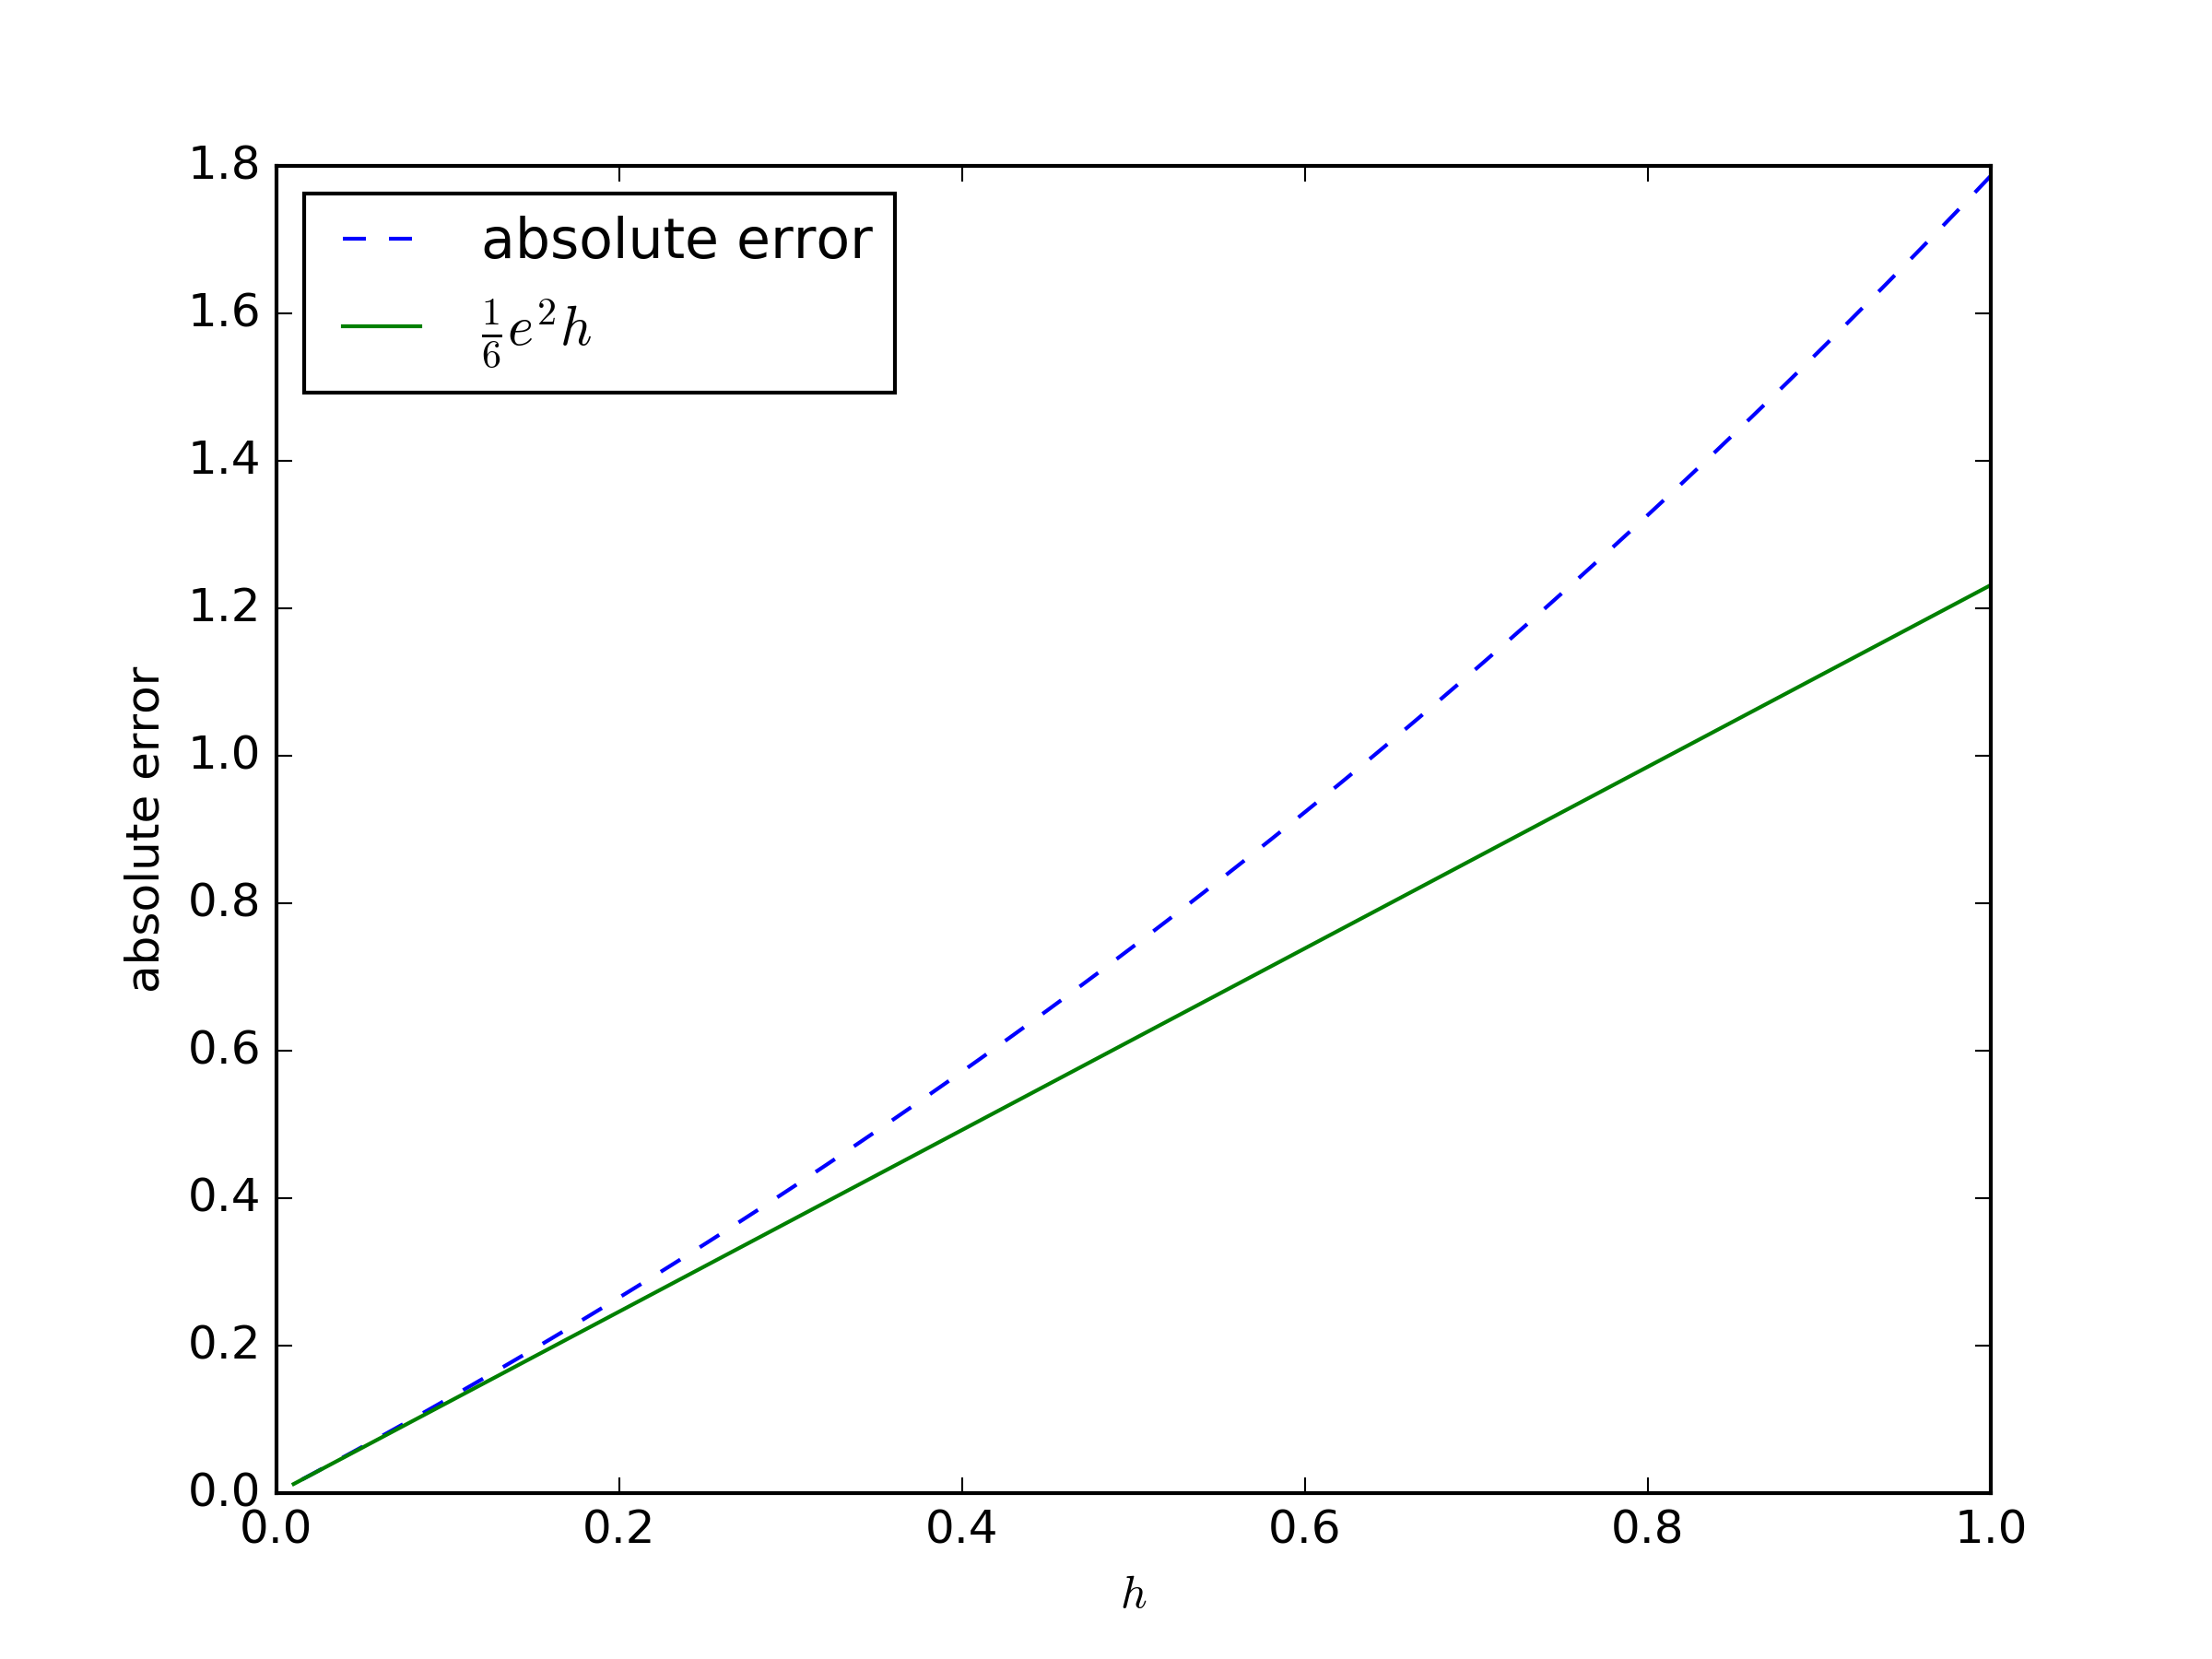
\includegraphics[scale=0.5]{problem_3.png}
        \end{figure}
    \pagebreak
    \item
        The polynomial through the points
        \begin{align*}
            (x,u(x)) \qquad (x + h, u(x+h)) \qquad \qty(x - \frac{h}{2}, u\qty(x - \frac{h}{2}))
        \end{align*}
        satisfies
        \begin{align*}
            u(x) &= A + Bx + Cx^2 \\
            u(x+h) &= A + B(x+h) + C(x+h)^2 \\
            u\qty(x - \frac{h}{2}) &= A + B\qty(x - \frac{h}{2}) + C\qty(x - \frac{h}{2})^2
        \end{align*}
        This is a simple linear algebra problem that can be solved symbolically using a symbolic solver like Maple or Python (\texttt{sympy} package).  We get:
        \begin{align*}
            A &= \frac{1}{3 h^{2}} \left(3 h^{2} u(x) + 4 h u\qty(x - \frac{h}{2}) x - 3 h u(x) x - h u\qty(x + h) x + 4 u\qty(x - \frac{h}{2}) x^{2} - 6 u(x) x^{2} + 2 u\qty(x + h) x^{2}\right) \\
            B &= -\frac{1}{3 h^{2}} \left(4 h u\qty(x - \frac{h}{2}) - 3 h u(x) - h u\qty(x + h) + 8 u\qty(x - \frac{h}{2}) x - 12 u(x) x + 4 u\qty(x + h) x\right) \\
            C &= \frac{2}{3 h^{2}} \left(2 u\qty(x - \frac{h}{2}) - 3 u(x) + u\qty(x + h)\right)
        \end{align*}
        Then note that since $u(x) = A + Bx + Cx^2$, then $u''(x) = 2C = \dfrac{8}{3h^2}u\qty(x - \dfrac{h}{2}) - \dfrac{4}{h^2}u(x) + \dfrac{4}{3h^2}u\qty(x + h)$, which exactly matches with the finite difference formula from part (a).  This means the best possible second derivative approximation using three points is precisely the quadratic function through those points.
\end{enumerate}

\end{document}









